\section{Comprensión y obtención de datos}
\label{sec:datos}

\subsection{Recolección de datos}

Los datos provienen de dos fuentes: la API pública de cotizaciones del dólar
blue \cite{dolarblue2026api} (nivel blue/oficial, series históricas y
microestructura P2P) y las normas publicadas en la Gaceta Oficial de Bolivia
\cite{gaceta2026}, en formato PDF. Los recolectores descargan ambas fuentes y
las persisten en \texttt{data/}; los datos se actualizan cada 24 horas.

Las normas se tipan con un modelo de lenguaje (LLM) que extrae de cada PDF
sus campos estructurados. El procesamiento posterior es reproducible y no
descarga nada: reconstruye la serie por hora \texttt{market\_hourly.csv}
(4\,318 horas observadas; 4\,321 en la grilla al interpolar el único hueco de
3~h) y el registro diario de normas \texttt{gaceta\_daily.csv} (181 días, con
cero en los días sin publicación; el panel de modelado conserva 179 porque
descarta los dos primeros días sin retorno previo). Ambos archivos
\textbf{conservan su resolución original} y no se remuestrean al recolectar:
la unión por fecha se hace en el paso de modelado, de modo que la misma capa
de datos sirve tanto al análisis por hora como al diario.

\begin{figure}[!ht]
\centering
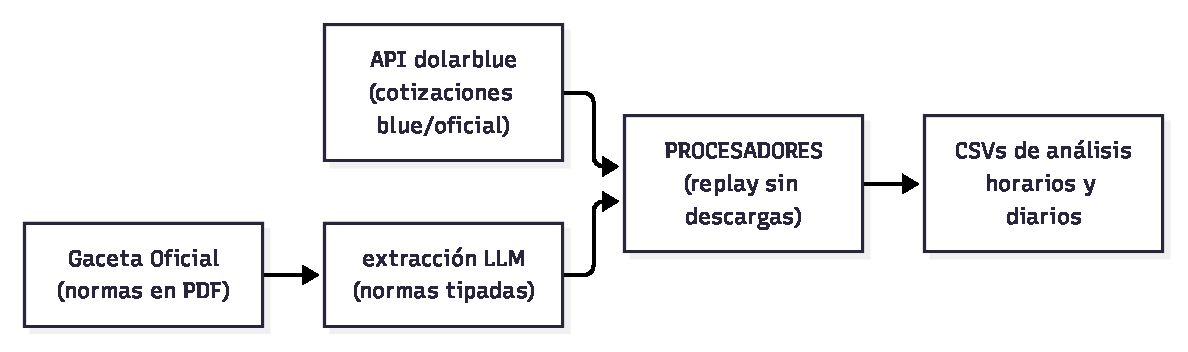
\includegraphics[width=\textwidth]{diagram_flujo_datos.pdf}
\caption{Obtención de datos: las dos fuentes convergen en los procesadores,
que producen los CSVs de análisis.}
\label{fig:flujo_datos}
\end{figure}

\subsection{Trazabilidad del pipeline}

La figura~\ref{fig:pipeline_anim} es el fotograma final de una animación de
60 segundos que recorre la extracción, los indexers y la exploración de las
dos fuentes. El video está en \texttt{report/anim/pipeline.mp4} (y la versión
GIF en \texttt{report/anim/pipeline.gif}); se regenera con
\texttt{make anim}.
Las escenas 5 y 6 detallan los dos indexers: el horario deriva precios medios,
spread, brecha, retorno y volatilidad; el diario construye un calendario
completo y rellena con cero los días sin publicación. La escena 7 muestra la
interpolación de huecos de hasta 3~h y las reglas para el resto. El notebook
(sección~2.2) y el dashboard (sección~3.6) reproducen las ocho escenas como
clips animados, con el frame final como respaldo.

La animación muestra el comportamiento efectivo del código. La corrida se
protege con un manifiesto de 24 h; cada PDF se reutiliza si ya está en disco
(más de 1~KB, validado por tamaño) y la extracción LLM se cachea por
\texttt{sha256(pdf):provider:model}; la firma \texttt{\%PDF} se exige en las
descargas nuevas. Un fallo de descarga o de esquema se
reintenta hasta tres veces con retroceso; si persiste, no se cachea y queda
para la corrida siguiente. La etiqueta \texttt{relevancia\_fx} es una salida:
una norma \texttt{nula} se conserva con peso cero y no se reintenta. En la
serie horaria, un único hueco de 3~h se interpola ($\le 3$~h); los huecos
mayores y el calentamiento de \texttt{vol\_24h} quedan como \texttt{NaN}, y
los días sin norma en la Gaceta son ceros estructurales, no datos faltantes.

\begin{figure}[!ht]
\centering
\includegraphics[width=\textwidth]{fig_pipeline_poster.pdf}
\caption{Fotograma final de la animación del pipeline: descarga única, cache
de extracción, reintento acotado y faltantes explícitos. El video completo
está en \texttt{report/anim/pipeline.mp4}.}
\label{fig:pipeline_anim}
\end{figure}

\subsection{Fuentes de datos}

Las fuentes del proyecto son la API pública de cotizaciones del dólar blue
\cite{dolarblue2026api} y las normas publicadas en la Gaceta Oficial de
Bolivia \cite{gaceta2026}.

La API expone tres categorías: cotizaciones al instante (nivel oficial y
libros P2P), series históricas por hora de 6 meses e historial completo
exportable.

\subsection{Diccionario de datos}

El modelado se alimenta de tres archivos. La tabla~\ref{tab:diccionario}
resume las variables que se usan y su unidad.

\begin{table}[!ht]
\centering\footnotesize
\begin{tabular}{@{}p{0.19\textwidth}p{0.34\textwidth}p{0.39\textwidth}@{}}
\toprule
Archivo & Variable & Contenido (unidad) \\
\midrule
\texttt{market\_hourly.csv} & & \emph{frecuencia horaria, 4\,318 filas} \\
 & \texttt{fecha} & marca horaria en UTC \\
 & \texttt{blue\_mid}, \texttt{oficial\_mid} & punto medio (compra$+$venta)/2
   del blue y del oficial (Bs/USD) \\
 & \texttt{brecha\_pct} & brecha blue--oficial sobre el oficial (\%) \\
 & \texttt{spread\_blue} & venta menos compra del blue (Bs/USD) \\
 & \texttt{ret\_blue\_1h} & retorno horario del blue (\%) \\
 & \texttt{vol\_24h} & desvío estándar móvil de 24~h de los retornos \\
\midrule
\texttt{panel\_diario.csv} & & \emph{179 días, cruce mercado $\times$ Gaceta} \\
 & \texttt{n\_docs\_fx}, \texttt{n\_docs\_fx\_alta} & normas del día con
   relevancia cambiaria media/alta y alta (conteo) \\
 & \texttt{n\_docs\_deuda}, \texttt{n\_docs\_comercio}, \texttt{n\_docs\_mineria}
   & normas del día por canal temático (conteo) \\
 & \texttt{vol\_media\_24h} & volumen P2P medio del día (USD) \\
 & \texttt{d\_oficial\_pct} & variación diaria del oficial (\%) \\
\midrule
\texttt{gaceta\_llm.csv} & & \emph{169 normas, una fila por documento} \\
 & \texttt{relevancia\_fx} & nula, baja, media o alta (categoría) \\
 & \texttt{tags} & canales temáticos asignados por el LLM \\
 & \texttt{monto\_usd} & monto explícito en dólares, si la norma lo declara \\
 & \texttt{confidence} & confianza de la extracción, entre 0 y 1 \\
\midrule
\emph{Derivadas} & \texttt{brecha\_lag1h}, \texttt{lag3h}, \texttt{lag24h},
   \texttt{oficial\_lag1h}, \texttt{vol\_lag1h}, \texttt{ret\_blue\_lag1h},
   \texttt{n\_docs\_*\_lag1} & rezagos usados como predictores (la Gaceta entra
   rezagada un día) \\
 & \texttt{hora\_*}, \texttt{dow\_*} & dummies de hora (23) y de día de la
   semana (6) \\
\bottomrule
\end{tabular}
\caption{Variables usadas por el modelado, por archivo.}
\label{tab:diccionario}
\end{table}

\subsection{Exploración (EDA)}
\label{sec:analisis}

La exploración usa la serie horaria de \textbf{4\,321 horas}
(2026-04-27 02:00 $\rightarrow$ 2026-10-24 02:00) y, para la brecha diaria,
la serie de \textbf{366 días} (2025-10-24 $\rightarrow$ 2026-10-24). El panel
que incorpora los canales de la Gaceta cubre \textbf{179 días}
(2026-04-29 $\rightarrow$ 2026-10-24).

\subsubsection{Serie blue vs oficial}

La \hyperref[fig:serie]{figura~\ref*{fig:serie}} muestra la serie por hora de
los últimos $\sim$6 meses (\texttt{chart\_6m.csv}): compra/venta del dólar
blue frente al oficial BCB. Se aprecia el tipo de cambio administrado (oficial
prácticamente plano) contra la flotación libre del paralelo.

\begin{figure}[!ht]
\centering
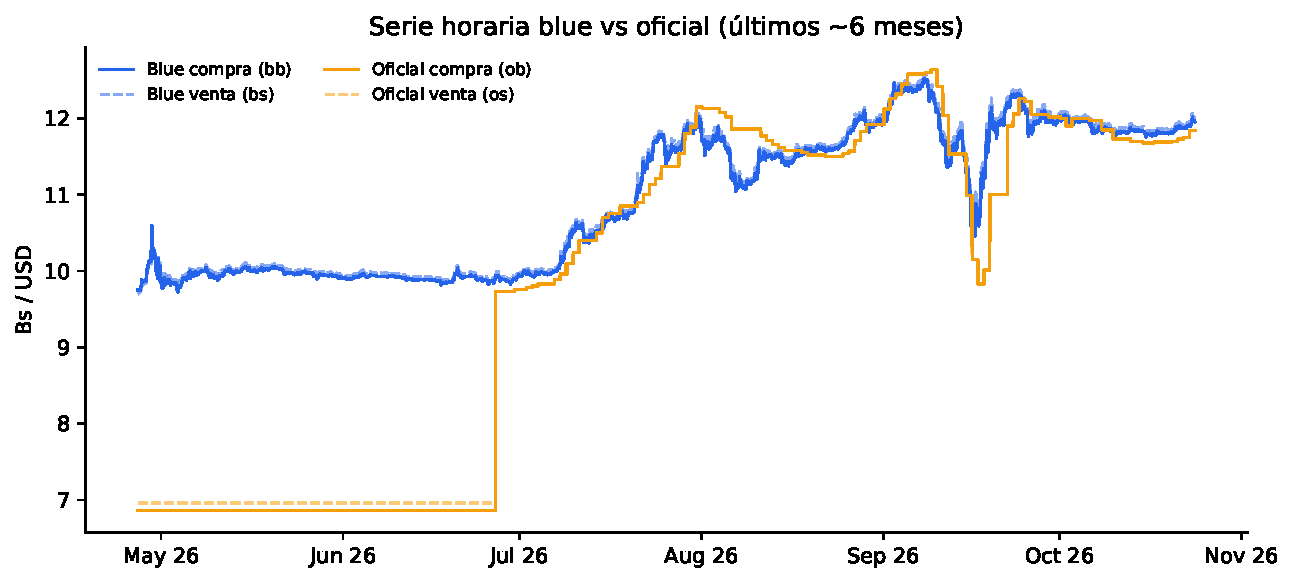
\includegraphics[width=\textwidth]{fig_serie_blue_oficial.pdf}
\caption{Serie por hora blue vs oficial (compra/venta), últimos $\sim$6 meses.}
\label{fig:serie}
\end{figure}

\subsubsection{La brecha cambiaria}

La \hyperref[fig:brecha]{figura~\ref*{fig:brecha}} resume la brecha diaria
(precio medio blue $-$ precio medio oficial) construida desde
\texttt{history\_full.csv} con resampleo diario. Es la base de la variable
objetivo de predicción (Objetivos 1--2, \hyperref[sec:preparacion]{sección~\ref*{sec:preparacion}}).

\begin{figure}[!ht]
\centering
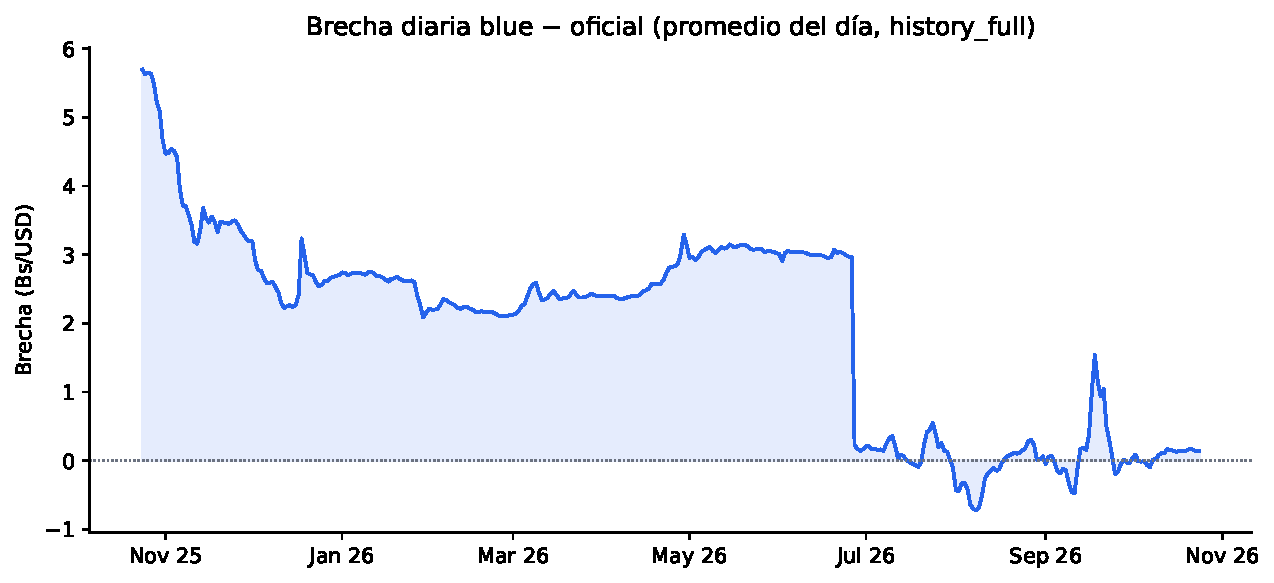
\includegraphics[width=\textwidth]{fig_brecha.pdf}
\caption{Brecha diaria blue $-$ oficial (promedio del día).}
\label{fig:brecha}
\end{figure}

\begin{table}[!ht]
\centering
% Generado por make_figures.py — no editar a mano
\begin{tabular}{@{}lll@{}}
\toprule
Métrica & Valor & Unidad \\
\midrule
Puntos horarios & 4.318 &  \\
Blue medio & 10,98 & Bs/USD \\
Oficial medio & 9,90 & Bs/USD \\
Spread blue medio (bs$-$bb) & 0,05 & Bs/USD \\
Volatilidad diaria blue ($\sigma$ de retornos) & 0,20 & \% \\
Días de brecha (history\_full) & 366 &  \\
Brecha media & 1,94 & Bs/USD \\
Brecha máxima & 5,70 & Bs/USD \\
\bottomrule
\end{tabular}

\caption{Métricas de la serie vigente (blue vs oficial, brecha y
volatilidad).}
\label{tab:resumen}
\end{table}


\subsection{Calidad de datos}

Sobre \textbf{34\,182 snapshots} se descartó un único registro con precio nulo;
la serie horaria requiere interpolar un único hueco de 3~h. La Gaceta tiene
\textbf{169 normas} extraídas con LLM (2026-06-18 $\rightarrow$ 10-20) más
\textbf{509} etiquetadas por palabras clave como respaldo (2025-10-12
$\rightarrow$ 10-07); aun así, solo \textbf{23 de los 179 días} del panel
tienen alguna norma con relevancia cambiaria. En el cruce temporal, 117 de los
249 pares fecha--tag del estudio de eventos tienen datos de mercado.
